\documentclass[12pt]{article}


\usepackage[utf8]{inputenc}
\usepackage[a4paper,top=3cm,bottom=2cm,left=3cm,right=3cm,marginparwidth=1.75cm]{geometry}
\usepackage[nodayofweek]{datetime}
\usepackage{tabularx}
\usepackage[small]{titlesec}
\usepackage{graphicx}
\usepackage{tabularx}

\newcolumntype{L}[1]{>{\raggedright\arraybackslash}p{#1}}
\newcolumntype{C}[1]{>{\centering\arraybackslash}p{#1}}
\newcolumntype{R}[1]{>{\raggedleft\arraybackslash}p{#1}}

\begin{document}

\begin{titlepage}
    \begin{center}
        \huge{\bfseries  Tribhuvan University}\\
        \Large{Institute of Engineering}\\
        \huge{ \bfseries  Pulchowk Campus}\\[3.2cm]


        \textsc{\Large Internet and Intranet}\\[-0.5cm]
        \line(1,0){400}\\
        \huge{\bfseries Lab 3}\\
        \large{Installation of Squid proxy server}
        \line(1,0){400}\\


        \textsc{\Large Submitted by:}\\
        \Large Bishal Katuwal\\ \large 075BCT028\\    [0.85cm]

        \textsc{\Large Submitted to:}\\\
        \large Department of Electronics and Computer Engineering\\Pulchowk Campus\\    [0.85cm]
        
        \textsc{\Large Submitted on:}\\
        \today
        
    \end{center}
\end{titlepage}
\pagebreak
% ===============================================================
\paragraph{\Large Title\\}
Installation of Squid proxy server

\paragraph{Background Theory\\}
A proxy server is a computer system or an application program that acts as an intermediary between client devices and the internet. It receives requests from clients, forwards them to the desired web servers, and returns the server's responses back to the clients.

Squid is an open-source proxy server that is commonly used for caching frequently accessed web content, filtering web traffic, and providing anonymity for clients. It can run on various platforms, including Linux, Windows, and macOS. Squid can be used as a forward proxy, allowing clients to make indirect network connections to other servers, or as a reverse proxy, serving as an intermediary for HTTP requests from clients to servers. Squid can also be used to control access to the internet, enforce security policies, and optimize network performance.

\paragraph{Activity}
\section{Installing Squid}
\begin{enumerate}
    \item Updated system packages.
    \begin{verbatim}
        sudo apt update
        sudo apt upgrade
    \end{verbatim}

    \item Installed squid proxy.
    \begin{verbatim}
        sudo apt install squid 
    \end{verbatim}

    \item Started and enabled squid.
    \begin{verbatim}
        sudo systemctl start squid
        sudo systemctl enable squid
    \end{verbatim}
\end{enumerate}
\begin{figure}[h!]
    \centering
    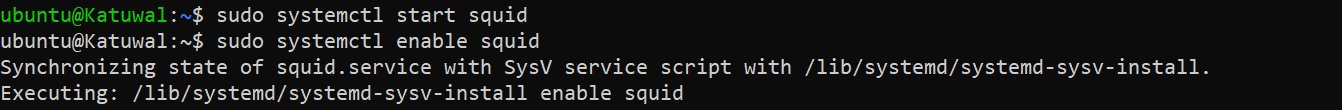
\includegraphics[scale = 0.70]{Images/start_squid.PNG}
    \caption{Docker installation}
\end{figure}

\section{Configuration of Squid proxy server}
\begin{enumerate}
    \item Configured squid.conf
    \begin{verbatim}
        sudo nano /etc/squid/squid.conf
    \end{verbatim}
    \item Replaced http\textunderscore access deny all with http\textunderscore access allow all.
    
    \begin{figure}[h!]
        \centering
        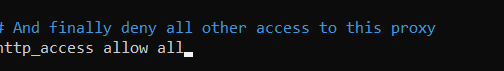
\includegraphics{Images/squid_access.PNG}
        \caption{HTML file}
    \end{figure}

    \item Restarted squid.
    \begin{verbatim}
        sudo systemctl restart squid
    \end{verbatim}
\end{enumerate}

\paragraph{Conclusion\\}
In this report, we have discussed the basic steps for Proxy Server configuration on Linux operating systems. 
The process of configuring proxy server in involves 
installing the squid software, 
configuring the squid.conf file for http\textunderscore access and 
ACL.

\end{document}